\documentclass[conference]{article}
%\IEEEoverridecommandlockouts
% The preceding line is only needed to identify funding in the first footnote. If that is unneeded, please comment it out.
\usepackage{algorithmic}
\hyphenation{op-tical net-works semi-conduc-tor IEEE-Xplore}
\def\BibTeX{{\rm B\kern-.05em{\sc i\kern-.025em b}\kern-.08em
    T\kern-.1667em\lower.7ex\hbox{E}\kern-.125emX}}
\usepackage[pdfencoding=auto, psdextra]{hyperref}
% \documentclass[]{amsart}
\usepackage{amsmath,amsfonts,amsthm}
\usepackage{mathtools}
\usepackage{tikz}
\usetikzlibrary{angles, quotes, patterns, backgrounds}  % Libraries in standalone file
\usepackage{float}

\usepackage{graphicx} % Required for inserting images
\DeclareMathOperator*{\argmin}{arg\,min}
\DeclareMathOperator*{\argmax}{arg\,max}
\newcommand{\matr}[1]{\bm{#1}}
\usepackage{bm}
\usepackage{cite}
\newcommand{\vect}[1]{\bm{#1}}
\theoremstyle{definition}
\newtheorem{theorem}{Theorem}
\newtheorem{corollary}{Corollary}[theorem] % Use theorem counter as `parent`
\newtheorem{defn}{Definition}[section]
\newtheorem{remark}{Remark}
\newtheorem{propn}[]{Proposition}
\newtheorem{lemma}[]{Lemma}
\newtheorem{proofpart}{Part}[theorem]
\renewcommand\theproofpart{\arabic{proofpart}}
\usepackage{bbm}
\usepackage{algorithmic}
\usepackage{calc}
\usepackage{array}
\usepackage{tabularx}
\usepackage{physics}

\usepackage{makecell}
\renewcommand\theadfont{\bfseries}

\usepackage[font=normalsize,labelfont=sf,textfont=sf]{subcaption}
\usepackage{textcomp}
\usepackage{stfloats}
\usepackage{url}
\usepackage{verbatim}
\usepackage{graphicx}
\usepackage{xcolor}
\usepackage{balance}
%\usepackage{hyperref}
\usepackage[pdfencoding=auto, psdextra]{hyperref}
\usepackage{booktabs}
\usepackage{cases}

%%%% Some specific notation
%% To Do: use msub to factor out these things
\usepackage{xstring}
\DeclareMathSymbol{\Theta}{\mathord}{operators}{"02}
\newcommand{\set}[1]{\mathcal{#1}}
%\newcommand{\set}[1]{\if1#1 \{1\}\else \mathcal{#1}\fi}
\newcommand{\sqfrob}[1]{\left|\left|#1\right|\right|^{2}_{F}}
\newcommand{\sqnormvec}[1]{\left|\left|#1\right|\right|^{2}_{2}}
%\newcommand{\trace}[1]{\textrm{tr}\left(#1\right)}
\NewDocumentCommand{\msub}{o o m}
{
    \IfValueT{#2}{\left[#3\right]_{\set{#1}, \set{#2}}}
    \IfNoValueTF{#1}{#3}{\left[#3\right]_{\set{#1}}}
}
\NewDocumentCommand{\msubgen}{o o m}
{
    \IfValueT{#2}{\left[#3\right]_{#1, #2}}
    \IfNoValueTF{#1}{#3}{\left[#3\right]_{#1}}
}
\NewDocumentCommand{\matrsub}{ o o m }
{
    \IfValueT{#2}{[\matr{#3}]_{\set{#1}, \set{#2}}}
    \IfNoValueTF{#1}{\matr{#3}}{[\matr{#3}]_{\set{#1}}}
}
\NewDocumentCommand{\matrsubpow}{ o o m m}
{
    \IfValueT{#2}{[\matr{#3}^{#4}]_{\set{#1}, \set{#2}}}
    \IfNoValueTF{#1}{\matr{#3}^{#4}}{[\matr{#3}^{#4}]_{\set{#1}}}
}
\NewDocumentCommand{\vectsub}{ o o m }
{
    \IfValueT{#2}{[\vect{#3}]_{\set{#1}, \set{#2}}}
    \IfNoValueTF{#1}{\vect{#3}}{[\vect{#3}]_{\set{#1}}}
}
%Optional arguments are for submatrix indexing
\NewDocumentCommand{\projbl}{ o o }
{
    \IfValueT{#2}{[\matr{\Pi}_{bl(\set{K})}]_{\set{#1},\set{#2}}}
    \IfNoValueTF{#1}{\matr{\Pi}_{bl(\set{K})}}{[\matr{\Pi}_{bl(\set{K})}]_{\set{#1}}}
}
%Optional arguments are for submatrix indexing
\NewDocumentCommand{\proj}{ o o m }
{
    \IfValueT{#2}{[\matr{\Pi}_{\set{#3}}]_{\set{#1}, \set{#2}}}
    \IfNoValueTF{#1}{\matr{\Pi}_{\set{#3}}}{[\matr{\Pi}_{\set{#3}}]_{\set{#1}}}
}
%As we do this so often
\newcommand{\matrsubU}[1]{\matrsub[#1, K]{U}}
\newcommand{\matrsubUGen}[1]{[\matr{U}]_{#1, \set{K}}}
\NewDocumentCommand{\expect}{ o m }
{
    \IfNoValueTF{#1}{{\mathbb{E}}\left[{{#2}}\right] }{{\mathbb{E}}_{#1}\left[{{#2}}\right]}
}
\NewDocumentCommand{\prob}{ o m }
{
    \IfNoValueTF{#1}{{\mathbb{P}}\left({{#2}}\right) }{{\mathbb{P}}_{#1}\left({{#2}}\right)}
}
\NewDocumentCommand{\expectnobig}{ o m }
{
    \IfNoValueTF{#1}{{\mathbb{E}}[{{#2}}] }{{\mathbb{E}}_{#1}[{{#2}}]}
}

\begin{document}

\title{Signs of Correlated Gaussians}

\author{{Baskaran Sripathmanathan} }
\maketitle


\begin{lemma}
\label{lemma:gaussian_sign}
Consider $\binom{X}{Y} \sim \mathcal{N}\left( \vect{0}, \begin{psmallmatrix} \sigma^{2} & c \\ c & \nu^{2} \end{psmallmatrix} \right)$. Let $\rho = \text{Corr}(X,Y) = \frac{c}{\sigma\nu}$. Then
\begin{equation}
    \mathbb{P}\left( X \text{ and } Y \text{ have different signs}\right) = \frac{ \text{arccos }\rho }{\pi}.
\end{equation}
    
\end{lemma}
\begin{proof}

 We first reduce to the case where $\sigma=\nu=1$. We see that $X' = \frac{X}{\sigma}, Y' = \frac{Y}{\nu}$ are $\mathcal{N}(0,1)$ with $\text{Cov}(X',Y') = \rho$ (by linearity of covariance). Note that $X$ and $Y$ have different signs $\iff XY < 0 \iff X'Y' < 0$; therefore $$\prob{X \text{ and } Y \text{ have different signs}} = \prob{X'Y' < 0}.$$

\noindent Now let $r = \frac{\rho}{\sqrt{1-\rho^2}}$ and $Z' = \frac{1}{\sqrt{1-\rho^{2}}}(\rho X' - Y')$. Then viewing $\binom{X'}{Z'}$ as a linear transformation of $\binom{X}{Y}$ (thus also multivariate gaussian), $\binom{X'}{Z'} \sim \mathcal{N}\left(\vect{0}, \matr{I}\right)$ and 
\begin{align}
 \prob{X'Y'<0} &= \prob{rX'^{2} < X'Z'} \\
 &= \prob{\{rX' < Z' \text{ and } X' > 0\} \cup \{rX' > Z' \text{ and } X' < 0 \}}   
\end{align}
 We depict this set as the shaded area in Figure \ref{fig:proof_fig}. 
\begin{figure}[H]
    \centering
    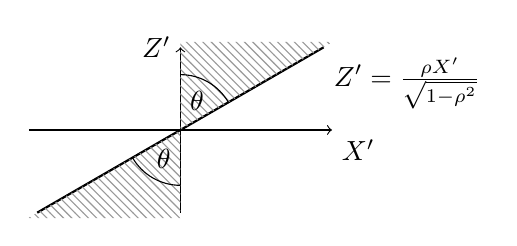
\begin{tikzpicture}[scale=0.35, background layer/.style={fill=none}]
% Define constants
\def\rhovalue{0.5}
\pgfmathsetmacro{\slope}{\rhovalue/sqrt(1-\rhovalue^2)}
\def\endX{5}
\pgfmathsetmacro{\endZ}{\slope*\endX}

% Draw axes
\draw[->] (0,-3) -- (0,3) node[left] {$Z'$};
\draw[->] (-5.5,0) -- (5.5,0) node[below right] {$X'$};

% Draw the line Z' = rho*X'/sqrt(1-rho^2) constrained within axis bounds
\pgfmathsetmacro{\leftX}{-3/\slope}  % X value where line reaches Z' = -3
\pgfmathsetmacro{\rightX}{3/\slope}  % X value where line reaches Z' = 3
\pgfmathsetmacro{\actualLeftX}{max(-5.5, \leftX)}
\pgfmathsetmacro{\actualRightX}{min(5.5, \rightX)}
\pgfmathsetmacro{\actualLeftZ}{\slope*\actualLeftX}
\pgfmathsetmacro{\actualRightZ}{\slope*\actualRightX}
\draw[thick] (\actualLeftX, \actualLeftZ) -- (\actualRightX, \actualRightZ) node[below right] {$Z' = \frac{\rho X'}{\sqrt{1-\rho^2}}$};
%\draw[thick] (\actualLeftX, \actualLeftZ) -- (\actualRightX, \actualRightZ) 
%  node[above right, xshift=-20pt, yshift=-10pt] {$Z' = \frac{\rho X'}{\sqrt{1-\rho^2}}$};


% Coordinates for angle measurement
\coordinate (O) at (0,0);
\coordinate (Zaxis) at (0,1);
\coordinate (LinePoint) at (1, \slope);
\coordinate (NegZaxis) at (0,-1);
\coordinate (NegLinePoint) at (-1, -\slope);
\coordinate (Zfar) at (0,3.2);
\coordinate (linetopfar) at (3.2/\slope, 3.2);
\coordinate (NegZfar) at (0,-3.2);
\coordinate (Neglinetopfar) at (-3.2/\slope, -3.2);

    \fill[pattern=north west lines, pattern color=black!40] 
      (O) -- (NegZfar) -- (Neglinetopfar) -- cycle;

    \fill[pattern=north west lines, pattern color=black!40] 
      (O) -- (Zfar) -- (linetopfar) -- cycle;

% Draw angle arc between Z' axis and the line
\pic[
    draw,
    angle radius=20pt,
    angle eccentricity=0.6,
    preaction={draw=white, line width=6pt},
    "$\theta$"
] {angle = LinePoint--O--Zaxis};


\pic[
    draw,
    angle radius=20pt,
    angle eccentricity=0.6,
    preaction={draw=white, line width=6pt},
    "$\theta$"
] {angle = NegLinePoint--O--NegZaxis};

\end{tikzpicture}
    \caption{$\{rX'^{2} < X'Z' \}$}
    \label{fig:proof_fig}
\end{figure}

Note that $\theta = \text{arccos}(\rho)$. The distribution of $\binom{X'}{Z'}$ is rotationally invariant, so if $\frac{n\pi}{\theta} \in \mathbb{Z}$, we can copy and rotate the shaded area $\frac{n\pi}{\theta}$ times to cover the plane (which corresponds to $\prob{X' \in \mathbb{R}, Z' \in \mathbb{R}} = 1$). Thus the shaded area is $\prob{X'Y'<0} = \frac{\theta}{\pi}$. Otherwise let $\theta_{n} = \frac{n\pi}{\left\lceil\frac{n\pi}{\theta} \right\rceil}$ and our argument applies if the shaded area were shrunk to $\theta_{n}$. Then $\theta_{n} \uparrow \theta$ as $n \to \infty$  and by countable additivity of measures, $\prob{X'Y' < 0} = \lim_{n\to\infty} \frac{\theta_{n}}{\pi} = \frac{\theta}{\pi}$.
\end{proof}

\end{document}